%%%%%%%%%%%%%%%%%%%%%%%%%%%%%%%%%%%%%%%%%%%%%%%%%%%%%%%%%%%%%%%%%%%%%%%%%%%%%%%%%%%
%% This project aims to create the UFC template for presentation.                %%
%% author: Maurício Moreira Neto - Doctoral student in Computer Science (MDCC)   %%
%% contacts:                                                                     %%
%%    e-mail: maumneto@ufc.br                                                    %%
%%    linktree: https://linktr.ee/maumneto                                       %%
%%%%%%%%%%%%%%%%%%%%%%%%%%%%%%%%%%%%%%%%%%%%%%%%%%%%%%%%%%%%%%%%%%%%%%%%%%%%%%%%%%%
\documentclass{libs/ufc_format}
% Inserting the preamble file with the packages
%%%%%%%%%%%%%%%%%%%%%%%%%%%%%%%%%%%%%%%%%%%%%%%%%%%%%%%%%%%%%%%%%%%%%
%% This file contains the packages that can be used in the beamer. %%
%%%%%%%%%%%%%%%%%%%%%%%%%%%%%%%%%%%%%%%%%%%%%%%%%%%%%%%%%%%%%%%%%%%%%
% Package to fonts family
\usepackage[T1]{fontenc}
% Package to accentuation
\usepackage[utf8]{inputenc}
% Package to Portuguese language
\usepackage[brazil]{babel}
% Package to Figures
\usepackage{graphicx}
% Package to the colors
\usepackage{color}
% Package to the colors
\usepackage{xcolor}
% Packages to math symbols and expressions
\usepackage{amsfonts, amssymb, amsmath}
% Package to multiple lines and columns in table
\usepackage{multirow, array} 
% Package to create pseudo-code
% For more detail of this package: http://linorg.usp.br/CTAN/macros/latex/contrib/algorithm2e/doc/algorithm2e.pdf
\usepackage{algorithm2e}
% Package to insert code
\usepackage{listings} 
\usepackage{keyval}
% Package to justify text
\usepackage[document]{ragged2e}
% Package to manage the bibliography
\usepackage[backend=biber, style=numeric, sorting=none]{biblatex}
% Package to facilities quotations
\usepackage{csquotes}
% Package to use multicols
\usepackage{multicol}

% Packages added by me
\usepackage{url}
\usepackage{tikz}
%\usepackage{multimedia}
%\usepackage{media9}[playbutton=plain, windowed=1280x720]
% Inserting the references file
\bibliography{references.bib}
\renewcommand*{\bibfont}{\scriptsize}

% Title
\title[ML]{\huge\textbf{Redes de Computadores}}
% Subtitle
\subtitle{}
% Author of the presentation
\author{Evandro J.R. Silva}
% Institute's Name
\institute[Estácio Teresina]{
    % email for contact
    \normalsize{\email{ejrs.profissional@gmail.com}}
    \newline
    % Department Name
    \department{Bacharelado em Ciência da Computação}
    \newline
    % university name
    %\ufc
    \estaciothe
}
% date of the presentation
\date{05 a 06 de Agosto}


%%%%%%%%%%%%%%%%%%%%%%%%%%%%%%%%%%%%%%%%%%%%%%%%%%%%%%%%%%%%%%%%%%%%%%%%%%%%%%%%%%
%% Start Document of the Presentation                                           %%               
%%%%%%%%%%%%%%%%%%%%%%%%%%%%%%%%%%%%%%%%%%%%%%%%%%%%%%%%%%%%%%%%%%%%%%%%%%%%%%%%%%
\begin{document}
% insert the code style
%%%%%%%%%%%%%%%%%%%%%%%%%%%%%%%%%%%%%%%%%%%%%%%%%%%%%%%%%%%%%%%%%%%%%%%%%%%%%%%%%%%
%% This file contains the style of the codes show in slides.                     %%
%% The package used is listings, but it possible to used others.                 %%
%%%%%%%%%%%%%%%%%%%%%%%%%%%%%%%%%%%%%%%%%%%%%%%%%%%%%%%%%%%%%%%%%%%%%%%%%%%%%%%%%%%

% color used in the code style
\definecolor{codegreen}{rgb}{0,0.6,0}
\definecolor{codegray}{rgb}{0.5,0.5,0.5}
\definecolor{codepurple}{rgb}{0.58,0,0.82}
\definecolor{codebackground}{rgb}{0.95,0.95,0.92}

% style of the code!
\lstdefinestyle{codestyle}{
    backgroundcolor=\color{codebackground},   
    commentstyle=\color{codegreen},
    keywordstyle=\color{magenta},
    numberstyle=\tiny\color{codegray},
    stringstyle=\color{codepurple},
    basicstyle=\ttfamily\footnotesize,
    frame=single,
    breakatwhitespace=false,         
    breaklines=true,                 
    captionpos=b,                    
    keepspaces=true,                 
    numbers=left,                    
    numbersep=5pt,                  
    showspaces=false,                
    showstringspaces=false,
    showtabs=false,                  
    tabsize=2,
    title=\lstname 
}

\lstset{style=codestyle}


%% ---------------------------------------------------------------------------
% First frame (with tile, subtitle, ...)
\begin{frame}{}
    \maketitle
\end{frame}

%% ---------------------------------------------------------------------------
% Second frame
\begin{frame}{Sumário}
    \begin{multicols}{2}
        \tableofcontents
    \end{multicols}
\end{frame}

%=============================================================================
% SECTION 1
%=============================================================================
\section{Introdução}

\begin{frame}{Introdução}
    \begin{itemize}
        \justifying
        \item O que é uma rede de computadores?
            \begin{itemize}
                \justifying
                \item<2-> É uma conexão entre, no mínimo, dois dispositivos.
            \end{itemize}
    \end{itemize}
\end{frame}

\begin{frame}{Introdução}
    \begin{itemize}
        \justifying
        \item Nos primórdios da computação (duas primeiras décadas):
    \end{itemize}
    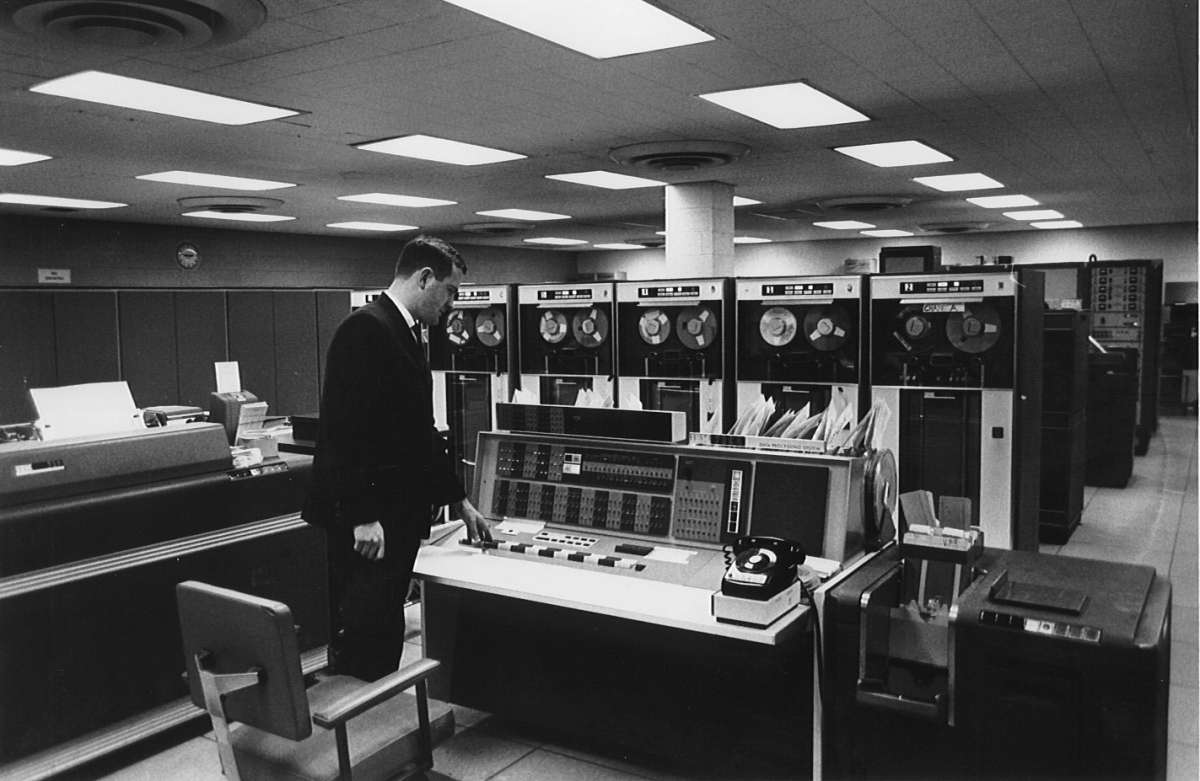
\includegraphics[width=\textwidth]{media/mainframe1}
\end{frame}

\begin{frame}{Introdução}
    \begin{itemize}
        \justifying
        \item Nos primórdios da computação (duas primeiras décadas):
    \end{itemize}
    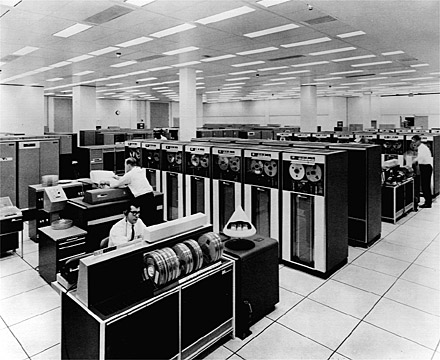
\includegraphics[height=7cm, width=\textwidth]{media/mainframe2}
\end{frame}

\begin{frame}{Introdução}
    \begin{itemize}
        \justifying
        \item Nos primórdios da computação (duas primeiras décadas):
    \end{itemize}
    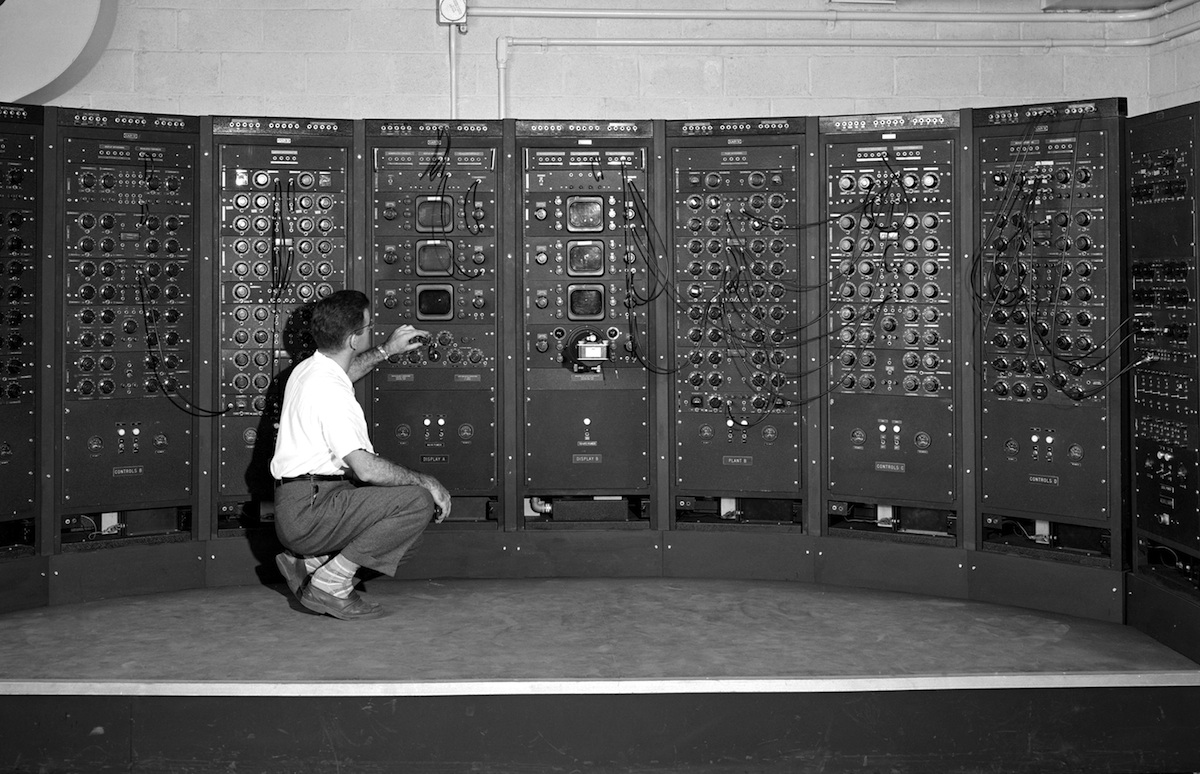
\includegraphics[width=\textwidth]{media/mainframe3}
\end{frame}

\begin{frame}{Introdução}
    \begin{itemize}
        \justifying
        \item Ou seja
    \end{itemize}
    \centering
    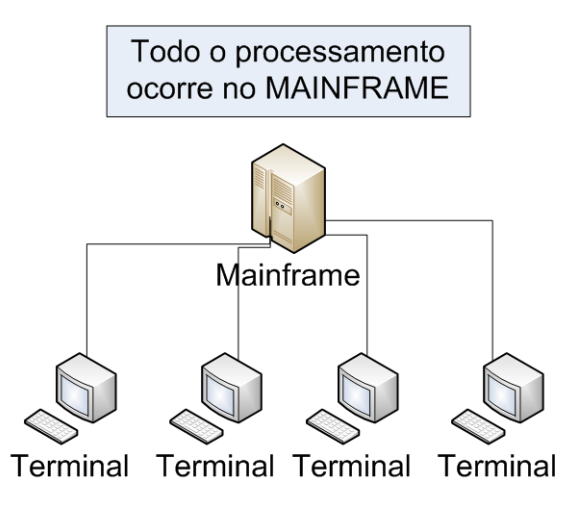
\includegraphics[scale=0.5]{media/mainframe4}
\end{frame}

\begin{frame}{Introdução}
    \begin{itemize}
        \justifying
        \item Os dispositivos em uma rede estão conectados através de um \textbf{enlace de comunicação}.
        \item<2-> A conexão era baseada em comutação de circuito\\
        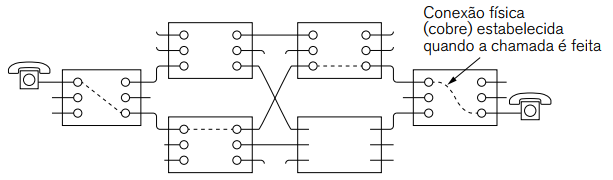
\includegraphics[width=10cm]{media/Comutação Circuito}
        \item<3-> Antes da comunicação os dispositivos reservavam recursos.
        \item<4-> Dados eram transferidos em um fluxo contínuo.
    \end{itemize}
\end{frame}

\begin{frame}{Introdução}
    \begin{itemize}
        \justifying
        \item Com o advento da \textbf{comutação de pacotes} a conectividade foi facilitada permitindo uma expansão das redes de computadores para uma escala global.
    \end{itemize}
    \centering
    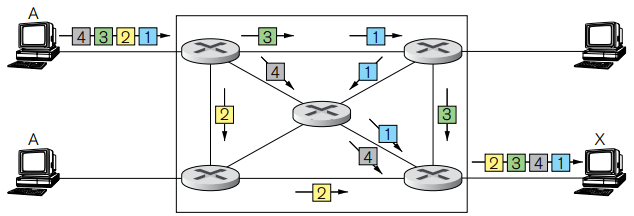
\includegraphics[width=\textwidth]{media/Comutação Pacote}
\end{frame}

\begin{frame}{Introdução}
    \begin{itemize}
        \justifying
        \item As redes podem conectar dispotivos através de:
            \begin{itemize}
                \item<2-> Fio de cobre;
                \item<3-> Fibra óptica;
                \item<4-> Microondas;
                \item<5-> Infravermelho;
                \item<6-> Satélites;
                \item<6-> etc.
            \end{itemize}
        \item<7-> Podem ter vários tamanhos e modelos.
        \item<8> \textbf{Internet}: uma rede de redes.
    \end{itemize}
\end{frame}

\begin{frame}{Introdução}
    \begin{itemize}
        \justifying
        \item Dois tipos gerais de transmissão
            \begin{itemize}
                \justifying
                \item<2-7> Enlace \textbf{ponto a ponto}
                    \begin{itemize}
                        \justifying
                        \item<3-7> Pares de máquinas conectadas;
                        \item<4-7> \textbf{Unicast} $\rightarrow$ quando não há rota entre os pontos.
                    \end{itemize}
                \item<2-7> Enlace \textbf{broadcast}
                    \begin{itemize}
                        \justifying
                        \item<5-7> Um pacote enviado por uma máquina é recebido por todas as outras máquinas;
                        \item<6-7> Um campo de endereço dentro do pacote especifica o destinatário;
                        \item<7> \textbf{Multicast} $\rightarrow$ quando um subconjunto de máquinas é o destinatário.
                    \end{itemize}
            \end{itemize}
            \item<8-> Elementos compartilhados pela rede
                \begin{itemize}
                    \item<9-> Dados;
                    \item<10-> Mensagens;
                    \item<11-> Impressoras;
                    \item<12-> Armazenamento;
                    \item<12-> etc.
                \end{itemize}
    \end{itemize}
\end{frame}

\begin{frame}{Introdução}
    \begin{itemize}
        \item Classificação das redes
            \begin{itemize}
                \item<2-> \alert<3>{Quanto a distância}.
                \item<2-> Quanto a topologia.
            \end{itemize}
    \end{itemize}
\end{frame}

\begin{frame}{Introdução}
    \begin{itemize}
        \item Classificação de redes quanto a distância
    \end{itemize}
    \centering
    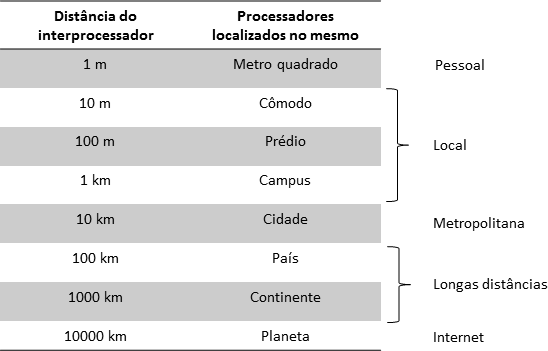
\includegraphics[scale=0.65]{media/clsredes}
\end{frame}

\begin{frame}{Introdução}
    \begin{itemize}
        \item Classificação de redes quanto a distância
            \begin{itemize}
                \item<1-2> \textit{Personal Area Network} (PAN)
                    \begin{itemize}
                        \justifying
                        \item<2> Bluetooth;
                        \item<2> RFID.
                    \end{itemize}
                \item<2-> \textit{Local Area Network} (LAN)
                    \begin{itemize}
                        \justifying
                        \item<3-> Rede particular com baixo a médio alcance.\\
                        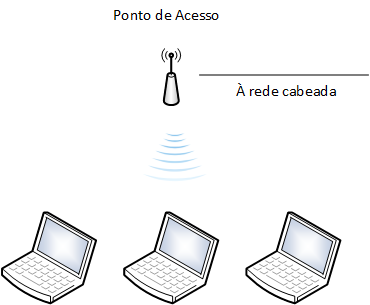
\includegraphics[width=0.35\textwidth, height=3.7cm]{media/wifi}
                        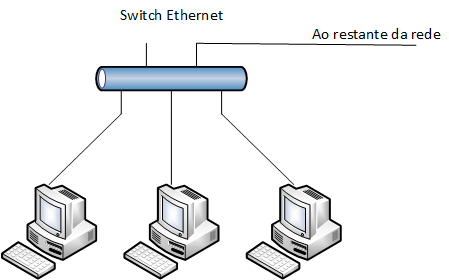
\includegraphics[width=0.45\textwidth, height=3.7cm]{media/ethernet}
                    \end{itemize}
            \end{itemize}
    \end{itemize}
\end{frame}

\begin{frame}{Introdução}
    \begin{itemize}
        \item Classificação de redes quanto a distância
            \begin{itemize}
                \item<1> \textit{Metropolitan Area Network} (MAN)\\
                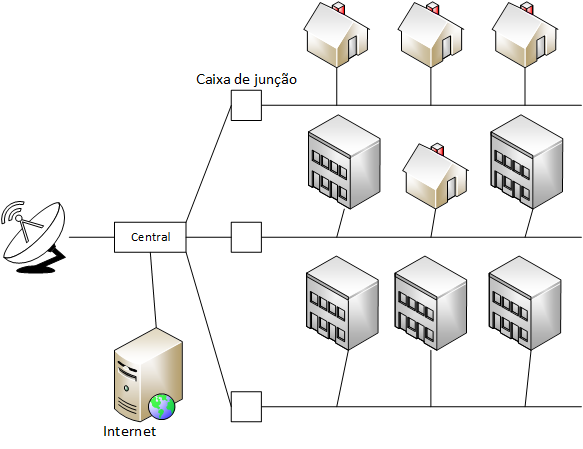
\includegraphics[width=0.7\textwidth, height=4.5cm]{media/man}
                \item<2-> \textit{Wide Area Network} (WAN)
                    \begin{itemize}
                        \justifying
                        \item<3-> Abrange uma ampla área geográfica.
                        \item<3-> Pode envolver países ou continentes.
                    \end{itemize}
            \end{itemize}
    \end{itemize}
\end{frame}

\begin{frame}{Introdução}
    \begin{itemize}
        \item Classificação das redes
            \begin{itemize}
                \item Quanto a distância.
                \item \alert{Quanto a topologia}.
            \end{itemize}
    \end{itemize}
\end{frame}

\begin{frame}{Introdução}
    \begin{itemize}
        \item Classificação de redes quanto a topologia
    \end{itemize}
    \centering
    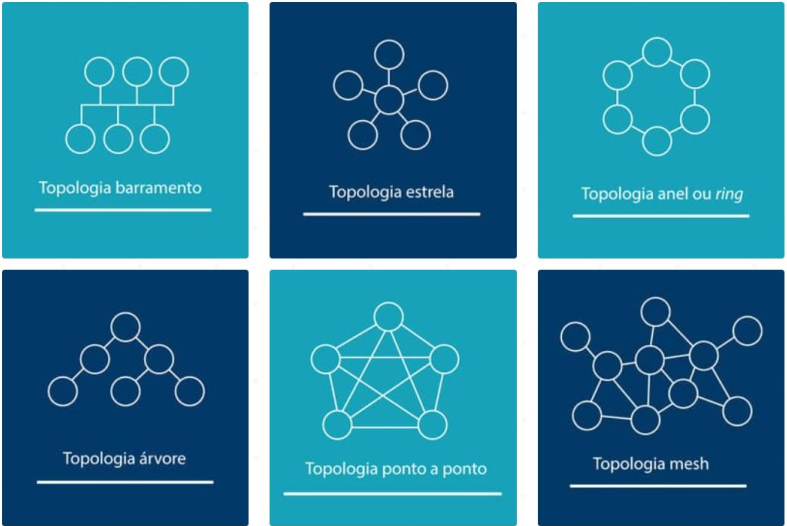
\includegraphics[width=\textwidth]{media/redes_topologia}
\end{frame}

%=============================================================================
% SECTION 2
%=============================================================================
\section{Modelo em Camadas}

\begin{frame}{}
    \centering
    \Large
    Modelo em Camadas
\end{frame}


\begin{frame}{Modelo em Camadas}
    \begin{itemize}
        \justifying
        \item Desde o início já se previa a comunicação entre dispositivos \textit{incomunicáveis}.
        \item Dispositivos diferentes, com arquiteturas diferentes, exigindo softwares diferentes.
        \item Fazê-los se comunicarem é uma tarefa complexa.
        \item<2-> Solução: dividir para conquistar!
            \begin{itemize}
                \justifying
                \item<3-> Em vez de soluções genéricas e complexas que cuidariam de todo o processo de comunicação, o processo deve ser subdividido.
                \item<4-> As redes passaram a ser divididas em camadas, onde em cada uma delas um determinado problema teria suas soluções.
            \end{itemize}
    \end{itemize}
\end{frame}

\begin{frame}{Modelo em Camadas}
    \centering
    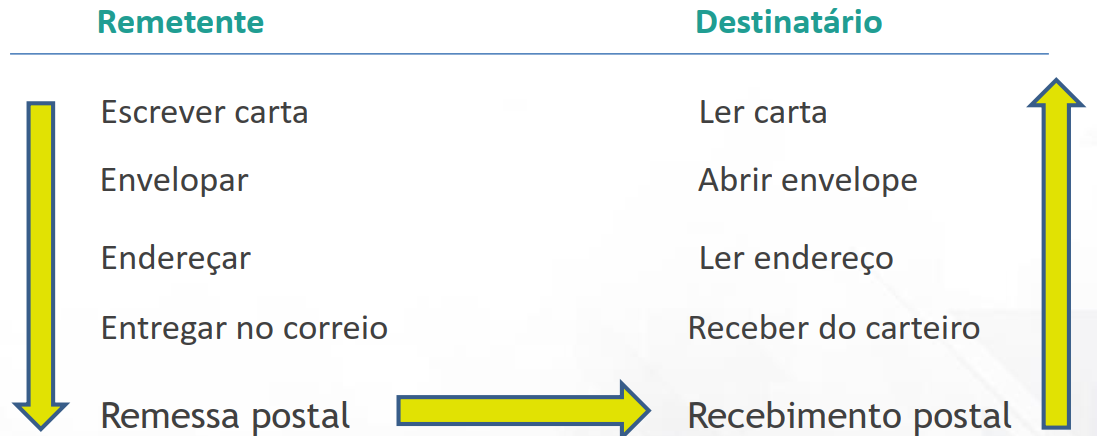
\includegraphics[width=\textwidth]{media/camadas_analogia}
\end{frame}

%-----------------------------------------------------------------------------
% SUBSECTION 2.1
%-----------------------------------------------------------------------------
\subsection{Modelo OSI}

\begin{frame}{}
    \centering
    \Large
    Modelo OSI
\end{frame}

\begin{frame}{Modelo OSI}
    \begin{itemize}
        \justifying
        \item O modelo OSI (\textit{Open Systems Interconnect}) foi criado, no fim da década de 1970, pela ISO (\textit{International Organization for Standardization}).
        \item O objetivo era estabelecer um padrão para que dispositivos de diferentes marcas pudessem se comunicar.
        \item O OSI acabou servido apenas de referência, já que não foi desenvolvido muito além do próprio modelo.
    \end{itemize}
\end{frame}

\begin{frame}{Modelo OSI}
    \begin{itemize}
        \item Princípios
            \begin{itemize}
                \justifying
                \item<2-3> Uma camada deve ser criada onde houver necessidade de outro grau de abstração.
                \item<3-4> Cada camada deve executar uma função bem definida.
                \item<4-5> A função de cada camada deve ser escolhida tendo em vista a definição de protocolos padronizados internacionalmente.
                \item<5-> Os limites de camadas devem ser escolhidos para minimizar o fluxo de informações pelas interfaces.
                \item<6-> O número de camadas deve ser grande o bastante para que funções distintas não precisem se desnecessariamente colocadas na mesma camada, e pequeno o suficiente para que a arquitetura não se torne difícil de controlar.
            \end{itemize}
    \end{itemize}
\end{frame}

\begin{frame}{Modelo OSI}
    \begin{columns}
        \begin{column}{0.45\textwidth}
            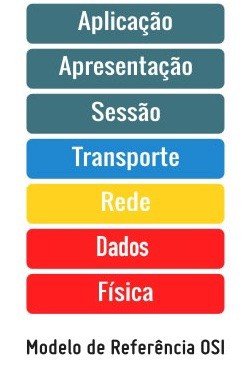
\includegraphics[width=\textwidth, height=0.8\textheight]{media/osi.jpeg}
        \end{column}
        
        \begin{column}{0.65\textwidth}
            \begin{itemize}
                \item Camada de Aplicação
                    \begin{itemize}
                        \justifying
                        \item<2> Onde devem estar aplicações específicas, como transferência de arquivos, correio eletrônico, login remoto, aplicações multimídias, etc.
                    \end{itemize}
                \item<3-> Camada de Apresentação
                    \begin{itemize}
                        \justifying
                        \item<4> Onde deve ocorrer a conversão adequada dos dados recebidos pela camada de Aplicação em um formato comum a ser usado na transmissão.
                    \end{itemize}
            \end{itemize}
        \end{column}
    \end{columns}
\end{frame}


\begin{frame}{Modelo OSI}
    \begin{columns}
        \begin{column}{0.45\textwidth}
            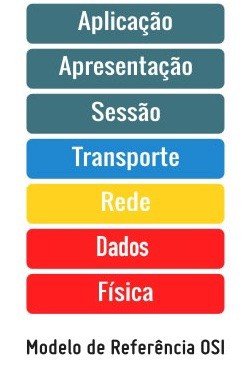
\includegraphics[width=\textwidth, height=0.8\textheight]{media/osi.jpeg}
        \end{column}
        
        \begin{column}{0.65\textwidth}
            \begin{itemize}
                \item Camada de Sessão
                    \begin{itemize}
                        \justifying
                        \item<2> Permite que usuários em diferentes máquinas estabeleçam sessões de comunicação.
                        \item<2> Oferece serviços de controle de diálogo, gerenciamento de tokens (para impedir que ambos os usuários tentem executar a mesma operação crítica ao mesmo tempo) e sincronização.
                    \end{itemize}
                \item<3-> Camada de Transporte
                    \begin{itemize}
                        \justifying
                        \item<4> Fornece comunicação \textit{fim a fim} com confiabilidade. Pode fornecer também controle do fluxo de dados, detecção e recuperação de erros. Caso seja necessário, divide os dados em unidades menores e garante que tais fragmentos cheguem corretamente à outra extremidade.
                    \end{itemize}
            \end{itemize}
        \end{column}
    \end{columns}
\end{frame}

\begin{frame}{Modelo OSI}
    \begin{columns}
        \begin{column}{0.45\textwidth}
            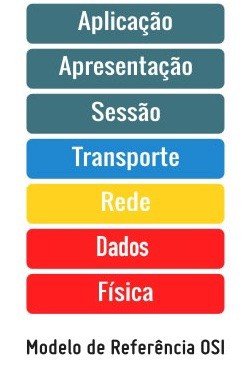
\includegraphics[width=\textwidth, height=0.8\textheight]{media/osi.jpeg}
        \end{column}
        
        \begin{column}{0.65\textwidth}
            \begin{itemize}
                \item Camada de Rede
                    \begin{itemize}
                        \justifying
                        \item<2> Determina a maneira como os pacotes são roteados da origem até o destino.
                        \item<2> Rotas podem ser tabelas estáticas --- com atualização automática --- ou dinâmicas --- de acordo com a carga atual da rede.
                        \item<2> Nesta camada pode haver o controle de congestionamento (gargalos).
                    \end{itemize}
                \item<3-> Camada de Enlace de Dados
                    \begin{itemize}
                        \justifying
                        \item<4> Detecta e, opcionalmente, corrige erros que ocorram no nível físico.
                        \item<4> Os dados vindos da camada superios são divididos em \textbf{quadros}.
                        \item<4> Controle de fluxo, para evitar que um transmissor mais rápido envie uma quantidade de dados excessiva a um receptor mais lento.
                    \end{itemize}
            \end{itemize}
        \end{column}
    \end{columns}
\end{frame}

\begin{frame}{Modelo OSI}
    \begin{columns}
        \begin{column}{0.45\textwidth}
            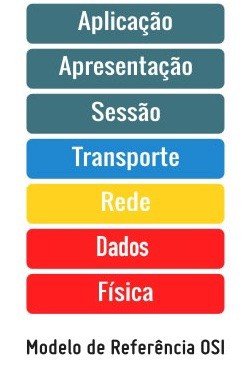
\includegraphics[width=\textwidth, height=0.8\textheight]{media/osi.jpeg}
        \end{column}
        
        \begin{column}{0.65\textwidth}
            \begin{itemize}
                \item Camada Física
                    \begin{itemize}
                        \justifying
                        \item<2> Transmite bits por um canal de comunicação.
                        \item<2> É onde se deve lidar com questões como:
                            \begin{itemize}
                                \justifying
                                \item<2> Quais sinais elétricos utilizar para representar os bits 0 e 1?
                                \item<2> Quanto tempo deve durar a representação de um bit?
                                \item<2> A transmissão pode acontecer em ambos os sentidos?
                            \end{itemize}
                    \end{itemize}
            \end{itemize}
        \end{column}
    \end{columns}
\end{frame}

\begin{frame}{Modelo OSI}
    \centering
    Resumo\\
    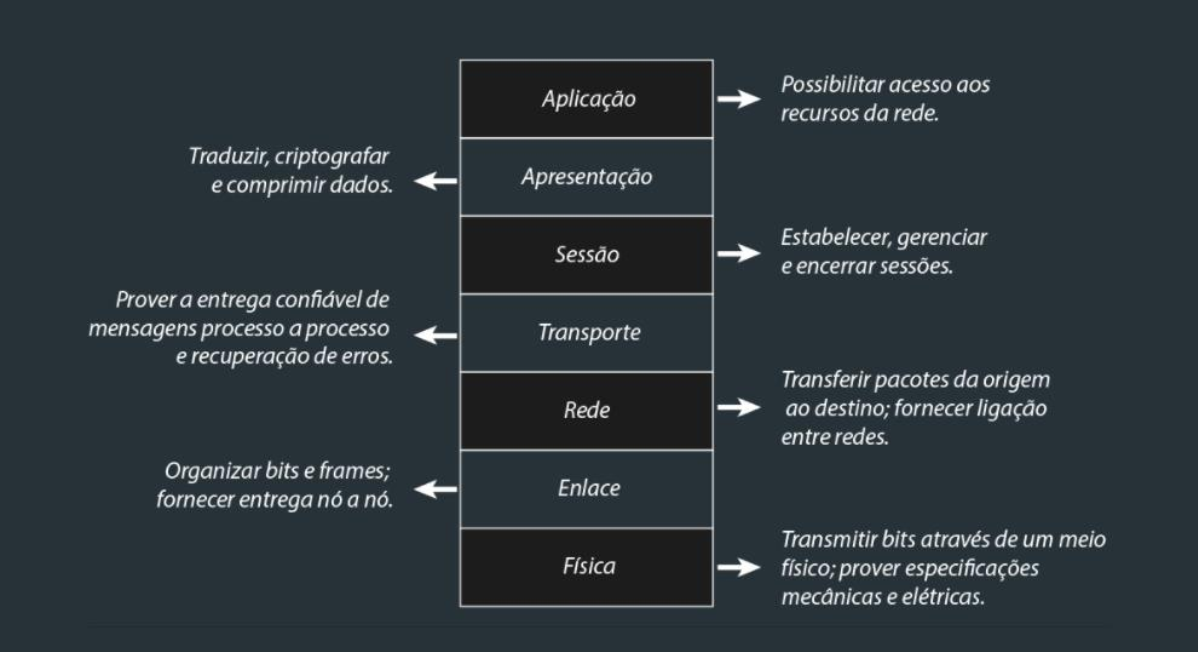
\includegraphics[width=\textwidth]{media/osi_resumo}
\end{frame}


%-----------------------------------------------------------------------------
% SUBSECTION 2.2
%-----------------------------------------------------------------------------
\subsection{TCP/IP}

\begin{frame}{}
    \centering
    \Large
    Arquitetura/Modelo TCP/IP
\end{frame}

\begin{frame}{TCP/IP}
    \begin{itemize}
        \justifying
        \item \textbf{ARPANET} (\textit{Advanced Research Projects Agency Network})
            \begin{itemize}
                \justifying
                \item É uma rede de computadores criada em 1969 para transmissão de dados militares sigilosos e interligação dos departamentos de pesquisa nos Estados Unidos.
                \item<2-> A rede foi crescendo, se juntando a ela outras universidades e repartições públicas.
                \item<3-> Com o advento das redes de rádio e satélites, os protocolos existentes começaram a ter problemas de interligação com elas.
                \item<4-> A partir daí foi construído uma arquitetura, que levou o nome de seus dois pincipais protocolos: TCP/IP.
            \end{itemize}
    \end{itemize}
\end{frame}

\begin{frame}{TCP/IP}
    \centering
    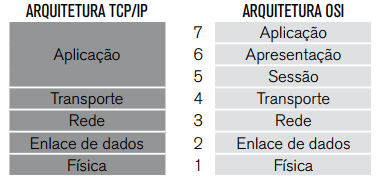
\includegraphics[width=\textwidth]{media/OSI e TCP}
\end{frame}

\begin{frame}{TCP/IP}
    \begin{itemize}
        \justifying
        \item Enquanto o modelo OSI especifica quais funções pertencem a cada uma de suas camadas, as camadas do conjunto de protocolos TCP/IP contêm protocolos relativamente independentes.
    \end{itemize}
    \centering
    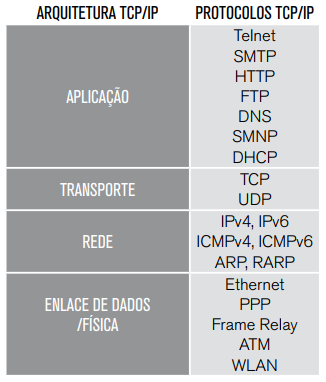
\includegraphics[scale=0.6]{media/TCP_IP}
\end{frame}

%=============================================================================
% SECTION 3
%=============================================================================
\section{Camada de Aplicação}

\begin{frame}{}
    \centering
    \Large
    Camada de Aplicação
\end{frame}

\begin{frame}{Princípio de Aplicações de Rede}
    \begin{itemize}
        \justifying
        \item Princípio básico: aplicativos / aplicações são programas que vão rodar em dispositivos diferentes e se comunicarem entre si.
        \item A duas principais arquiteturas de aplicação: cliente-servidor e sistema P2P.
    \end{itemize}
\end{frame}

%-----------------------------------------------------------------------------
% SUBSECTION 3.1
%-----------------------------------------------------------------------------
\subsection{Arquiteturas de aplicação de rede}

\begin{frame}{Arquiteturas de aplicação de rede}
    \begin{itemize}
        \item \textbf{Arquitetura cliente-servidor}
            \begin{itemize}
                \justifying
                \item Existe um hospedeiro (\textbf{servidor}) que está sempre em funcionamento.
                \item<2-> Outros hospedeiros (\textbf{clientes}) fazem requisições constantes ao servidor. Perceba que os clientes não se comunicam diretamente!
                \item<3-> Algumas aplicações \textit{gerais} que utilizam esta arquitetura: Web, FTP, Telnet, email ...
                \item<4-> Alguns exemplos mais específicos: Jogos online (fps, mmorpg, etc.); Redes Sociais; Sites (serviços públicos ou privados);
                \item<5-> O endereço (IP) do servidor é bem conhecido, ou seja, um servidor está sempre disponível para os clientes se conectarem.
                \item<6> E o que acontece se um servidor recebe mais requisição do que pode suportar?
            \end{itemize}
    \end{itemize}
\end{frame}

\begin{frame}{Arquiteturas de aplicação de rede}
    \centering
    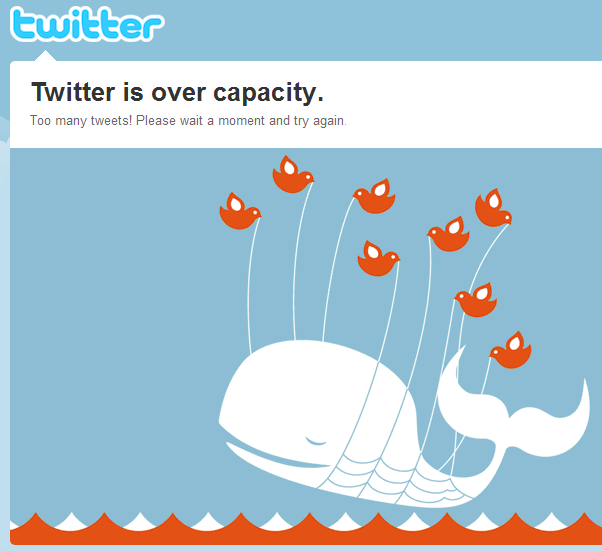
\includegraphics[scale = 0.5]{figuras/figura02_01}
\end{frame}

\begin{frame}{Arquiteturas de aplicação de rede}
    \begin{itemize}
        \item \textbf{Arquitetura P2P}
            \begin{itemize}
                \justifying
                \item Comunicação direta entre duplas (\textbf{pares}, \textit{peer} em Inglês) de hospedeiros.
                \item<2-> Podem gerar tráfego intenso! (Terror das ISPs)
                \item<3-> Uma das aplicações mais conhecidas: \textit{torrent}.\\
                \centering
                
\includegraphics[scale = 0.1]{figuras/figura02_04}
                \item<4-> Possui \textbf{autoescalabilidade}, à medida em que novos pares ficam disponíveis.
                \item<5-> Como não depende da potência de um servidor, o tráfego é \textit{distribuído}.
            \end{itemize}
    \end{itemize}
\end{frame}

\begin{frame}{Arquiteturas de aplicação de rede}
    \begin{itemize}
        \item \textbf{Arquitetura P2P}
            \begin{itemize}
                \item Principais desafios
                    \begin{enumerate}
                        \justifying
                        \item<2-> ISPs ficarem ok com isso. A infraestrutura é pressionada. Aqui temos 2 problemas: (1) taxa de \textit{upload} normalmente muito menor que a de \textit{download} e (2) o usuário consegue topar sua largura de banda. Lembrando que no contrato ISPs não são obrigadas a entregar 100\% da velocidade. Isto permite às empresas ter um \textit{excedente} de clientes em cada link.
                        \item<3-> Segurança.
                        \item<4-> Incentivos da / para a comunidade de usuários (\textit{comunidades de torrent fechadas}).
                    \end{enumerate}
            \end{itemize}
    \end{itemize}
\end{frame}

%-----------------------------------------------------------------------------
% SUBSECTION 3.2
%-----------------------------------------------------------------------------
\subsection{Comunicação entre processos}

\begin{frame}{Comunicação entre processos}
    \begin{itemize}
        \justifying
        \item O termo mais técnico para um programa é \textit{processo}. Os programas em execução na máquia são processos gerenciados pelo SO. A comunicação entre dois dispositivos é feita através de processos.
        \item Tipos de processos na rede
            \begin{itemize}
                \justifying
                \item<2> \textbf{Cliente} : processo que inicia a comunicação, envia as requisições.
                \item<2> \textbf{Servidor} : processo que recebe as requisições.
            \end{itemize}
    \end{itemize}
\end{frame}

\begin{frame}{Interface entre o processo e a rede}
    \begin{itemize}
        \justifying
        \item Um processo envia e recebe mensagens através de uma interface denominada \textbf{\textit{socket}}.
    \end{itemize}
    \centering
    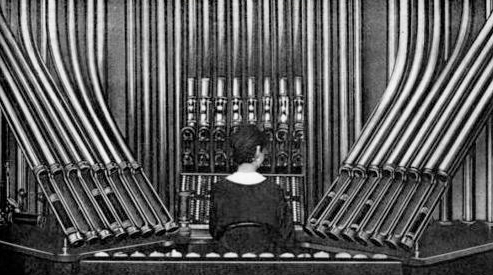
\includegraphics[scale = 0.5]{figuras/figura02_02_01}
\end{frame}

\begin{frame}{Interface entre o processo e a rede}
    \begin{itemize}
        \justifying
        \item O programador tem controle apenas sobre a Camada de Aplicação. Porém, pode acontecer o caso de poder escolher o Protocolo da Camada de Transporte e alguns parãmetros como tamanho do \textit{buffer} e segmentos.
    \end{itemize}
    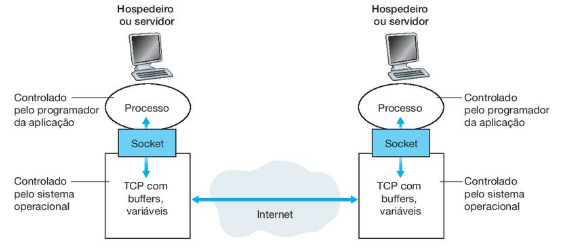
\includegraphics[scale = 0.75]{figuras/figura02_03}
\end{frame}

\begin{frame}{Interface entre o processo e a rede}
    \begin{itemize}
        \justifying
        \item Quando o processo envia a mensagem, o enderçamento deve conter, além do IP, o \textbf{número de porta} (que serve como um \textit{socket receptor}.
    \end{itemize}
\end{frame}
%=============================================================================
% SECTION REFERENCES
%=============================================================================
%\begin{frame}[allowframebreaks]{Referências}
%    \scriptsize
%    \printbibliography
%\end{frame}

\end{document}













%% ---------------------------------------------------------------------------
% This presentation is separated by sections and subsections
%\section{Seção I}
%\begin{frame}{Explicações}
%    % itemize
%    Este é um template que pode ser utilizado para:
%    \begin{itemize}
%        \item Apresentação de Trabalhos Acadêmicos
%        \item Apresentação de Disciplinas
%        \item Apresentações de Teses e Dissertações
%    \end{itemize}
%
%    \vspace{0.4cm} % vertical space
%    
%    % enumeration
%    Para utilizar este template corretamente é importante que:
%    \begin{enumerate}
%        \item Tenha conhecimento mínimo sobre LaTeX
%        \item Ler os comentários no template (explicações)
%        \item Ler o README.md (documentação)
%    \end{enumerate}
%
%    \vspace{0.2cm}

%    \example{Este é um texto de exemplo!} \emph{Texto de Ênfase!}
%\end{frame}

%% ---------------------------------------------------------------------------
%\subsection{Subseção I}
%\begin{frame}{Criando Blocos}
%    % Blocks styles
%    \begin{block}{Bloco Padrão}
%        Texto do corpo do bloco.
%    \end{block}

%    \begin{alertblock}{Bloco de Alerta}
%        Texto do corpo do bloco.
%    \end{alertblock}
%
%    \begin{exampleblock}{Bloco de Exemplo}
%        Texto do corpo do bloco.
%    \end{exampleblock}   
%\end{frame}

%% ---------------------------------------------------------------------------
%\subsection{Subseção II}
%\begin{frame}{Criando Caixas}
%    \successbox{testando o success box}
%
%    \pause
%
%    \alertbox{testando o alert box}
%
%    \pause
%
%    \simplebox{testando o simple box}
%\end{frame}

%% ---------------------------------------------------------------------------
%\subsection{Subseção III}
%\begin{frame}{Criando Algoritmos (Pseudocódigo)}
%    \begin{algorithm}[H]
%        \SetAlgoLined
%        \LinesNumbered
%        \SetKwInOut{Input}{input}
%        \SetKwInOut{Output}{output}
%        \Input{x: float, y: float}
%        \Output{r: float}
%        \While{True}{
%          r = x + y\;
%          \eIf{r >= 30}{
%           ``O valor de $r$ é maior ou iqual a 10.''\;
%           break\;
%           }{
%           ``O valor de $r$ = '', r\;
%          }
%         } 
%         \caption{Algorithm Example}
%    \end{algorithm}
%\end{frame}

%% ---------------------------------------------------------------------------

%\begin{frame}{Inserindo Algoritmos}
%    \lstset{language=Python}
%    \lstinputlisting[language=Python]{code/main.py}
%\end{frame}

%% ---------------------------------------------------------------------------
%\begin{frame}{Inserindo Algoritmos}
%    \lstinputlisting[language=C]{code/source.c}
%\end{frame}

%% ---------------------------------------------------------------------------
%\begin{frame}{Inserindo Algoritmos}
%    \lstinputlisting[language=Java]{code/helloworld.java}
%\end{frame}

%% ---------------------------------------------------------------------------
%\begin{frame}{Inserindo Algoritmos}
%    \lstinputlisting[language=HTML]{code/index.html}
%\end{frame}

%% ---------------------------------------------------------------------------
% This frame show an example to insert multicolumns
%\section{Multicolunas}
%\begin{frame}{Seção II - Multicolunas}
%    \begin{columns}{}
%        \begin{column}{0.5\textwidth}
%            \justify
%            É possível colocar mais de uma coluna utilizando os comandos de $\backslash$begin\{column\}\{\} e $\backslash$end\{column\}
%        \end{column}
%        \begin{column}{0.5\textwidth}
%            \justify
%            Porém, o espaçamento deve ser proporcional entre as colunas para que estas colunas não entrem em coflito. O espaçamento é dado pelo segundo argumento do $\backslash$begin.
%        \end{column}
%    \end{columns}    
%\end{frame}

%% ---------------------------------------------------------------------------
% This frame show an example to insert figures
%\section{Imagens}
%\begin{frame}{Seção III - Figures}
%    \begin{figure}
%        \centering
%        \caption{Emblema da UFC.}
%        
\includegraphics[scale=0.3]{libs/emblemufc.pdf}
%        \source{Obtido pelo site oficial da UFC \cite{siteufc} \cite{einstein}}
%        \label{fig:ufc_emblem}
%    \end{figure}
%\end{frame}

%% ---------------------------------------------------------------------------
% Reference frames
%\begin{frame}[allowframebreaks]
%    \frametitle{Referências}
%    \printbibliography
%\end{frame}

%% ---------------------------------------------------------------------------
% Final frame
%\begin{frame}{}
%    \centering
%    \huge{\textbf{\example{Obrigado(a) pela Atenção!}}}
%    
%    \vspace{1cm}
%    
%    \Large{\textbf{Contato:}}
%    \newline
%    \vspace*{0.5cm}
%    \large{\email{usuario@dominio}}
%\end{frame}